%%%%%%%%%%%%%%%%%%%%%%%%%%%%%%%		CHAP 5		%%%%%%%%%%%%%%%%%%%%%%%%%%%%%%%

\chapter{Data analysis results}
\label{cha:analysis}

 Some data analysis results are presented in this chapter, regarding either the method developed or simulation.
 The plots reported here were realised using the $C$ data set.


\section{Cosmic muons}
\label{sec:cosmic}

 High energy particles, mainly originated outside the Solar System and thus called %
 \emph{Cosmic Rays}, impact on the Earth's atmosphere and producing mesons, which in turn generate %
 secondary particle shower by decaying.
 The primary particles are about 99\,\% made of ionised nuclei (whose 86\,\% made of protons, %
 \np{12.7}\,\% of helium nuclei, and \np{1.3}\,\% of heavier nuclei), while the remaining 1\,\% is mostly %
 composed by electrons cite[theodorsson].
 The intensity of the nucleons in the energy range from several GeV to somewhat beyond 100 TeV %
 is given approximately by
 \begin{equation}
   \label{eq:cosmicI}
   I_N(E) \simeq \np{1.8e4} (\frac{E}{1~Gev})^{-\alpha}~\mathrm{\frac{nucleons}{m^2\,s\,sr\,Gev}}\,,
 \end{equation}
 where $E$ is the energy-per-nucleon, including rest mass energy, and $\alpha = \gamma +1 = \np{2.7}$ %
 is the differential spectral index of the cosmic ray flux, with $\gamma$ the integral spectral %
 index.

 %\begin{figure}[]
\begin{wrapfigure}{R}{0.5\textwidth}
   \centering
   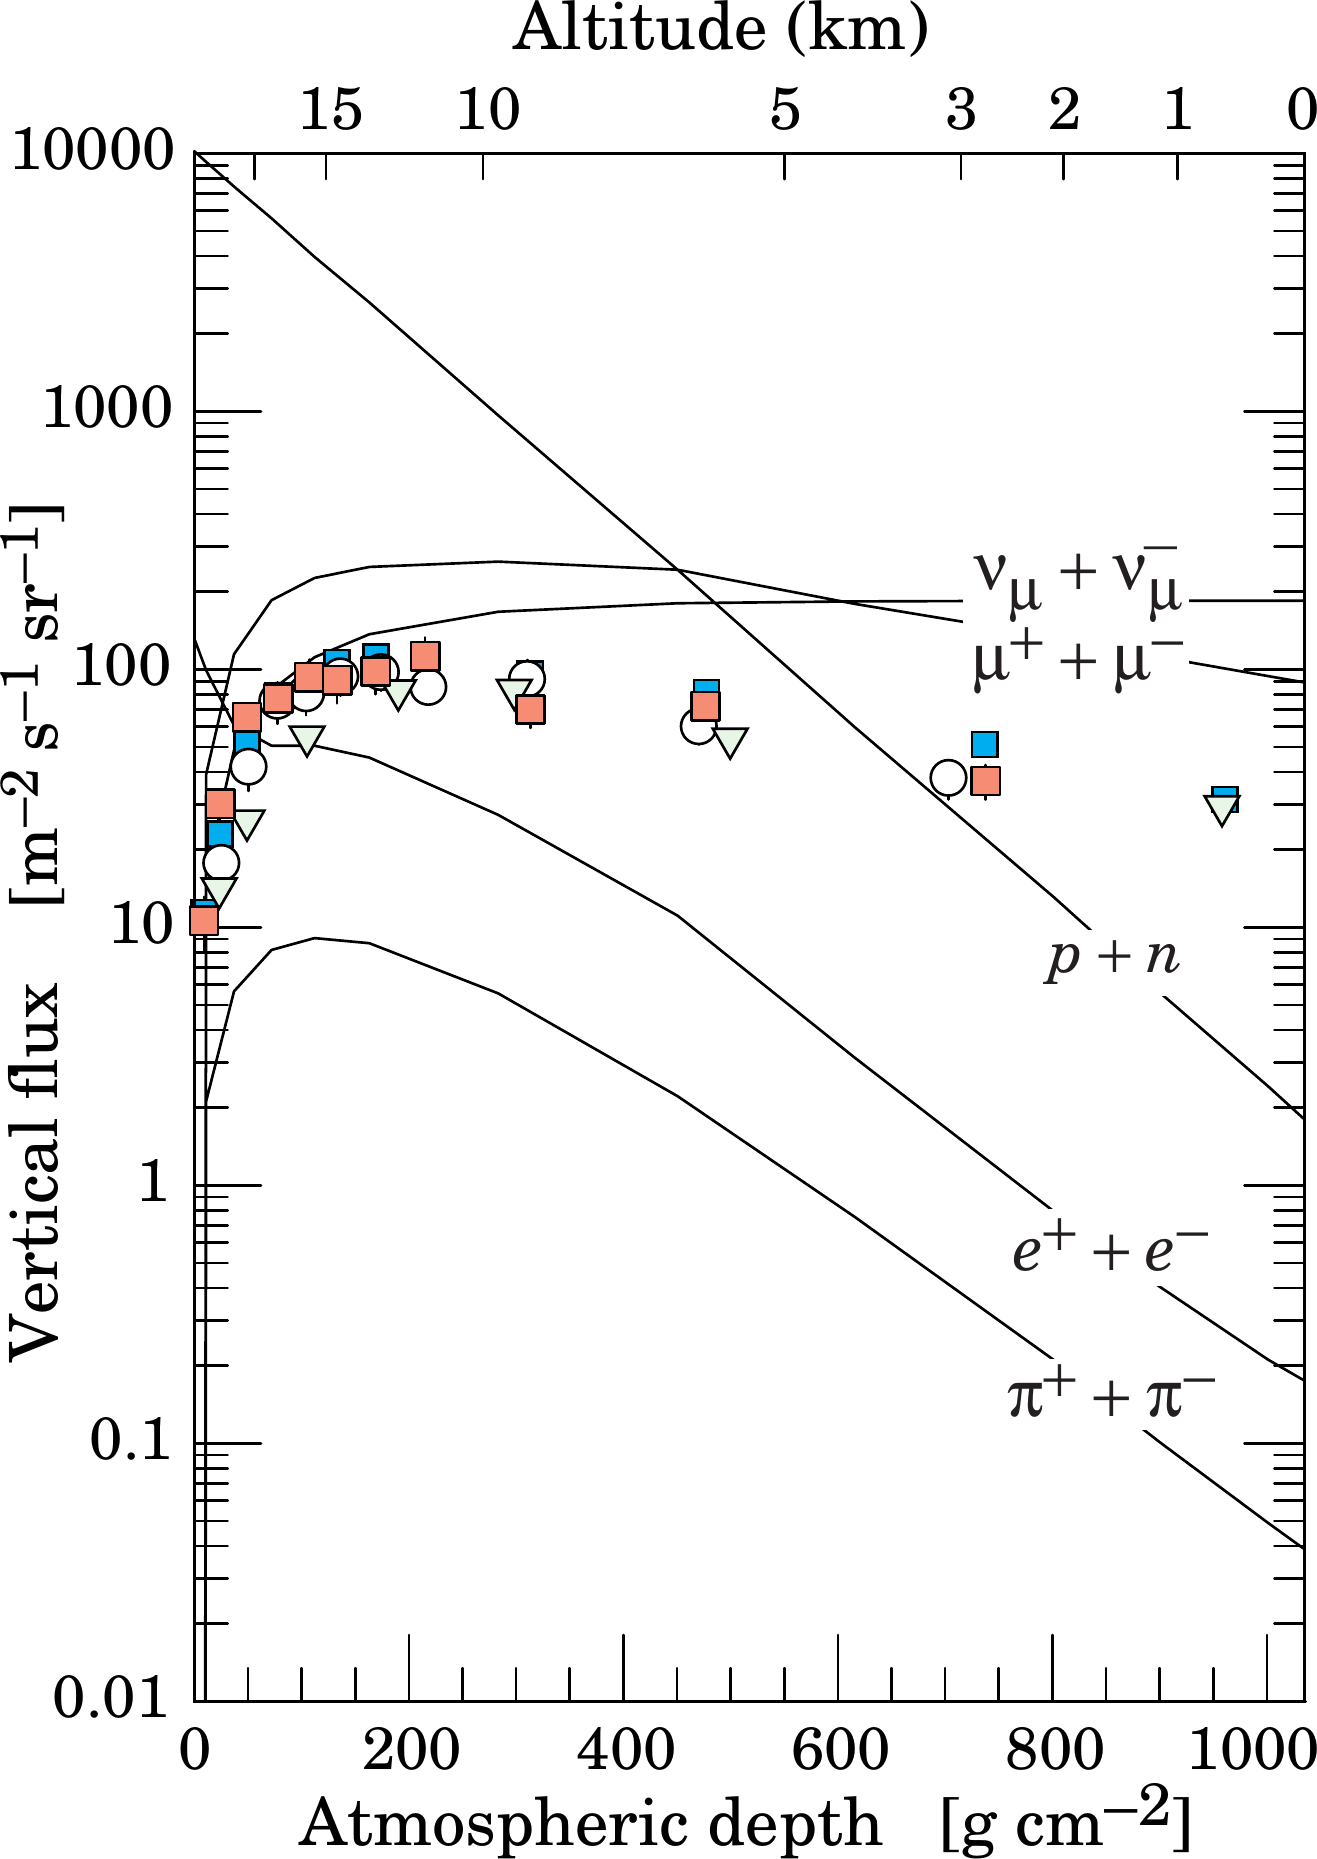
\includegraphics[scale=0.20]{pics/muonflux}
   \caption{Vertical fluxes of cosmic rays in the atmosphere with $E > 1$~GeV estimated %
     from the nucleon flux of Eq.~\ref{eq:cosmicI}. The points show measurements of negative muons %
     with 1 GeV from~ref[32–36].}
   \label{fig:muonflux}
 %\end{figure}
\end{wrapfigure}

 Many are the secondary products reaching the sea level, among which muons, neutrinos, nucleons, and %
 electrons.
 The first two, muons and neutrinos, derive from the decay chain of charged mesons, while electrons %
 and photons originate in decays of neutral mesons.
 As Fig.~\ref{fig:muonflux} shows, muons are the most numerous charged particles at sea level.
 Their direction of propagation is the same as that of their parents pions and in average they receive close %
 to 80\,\% of their parent's energy.
 They are very penetrating as their nuclear interaction cross section is only about $\np{2e-29}~\mathrm{cm}^2$ %
 (or two microbarns).
 The energy loss to ionisation is at a fairly constant rate of about 2~MeV per g/cm$^2$.
 Given that the vertical depth of the atmosphere is about 1000~g/cm$^2$, muons will lose about two~GeV %
 before reaching the ground. 
 The mean energy of muons at sea level is about four~GeV; therefore the mean energy at creation, %
 typically fifteen kilometres high, is probably near six~GeV.
 Their energy and angular distribution reflect a convolution of the production spectrum, %
 energy loss in the atmosphere, and decay. 
 %The energy spectrum is almost flat below 1 GeV, steepens gradually to reflect the primary %
 %spectrum in the 10$\div$100~GeV range, and steepens further at higher energies because pions %
 %with $E_\pi > \epsilon_\pi$ tend to interact in the atmosphere before they decay, where %
 %$\epsilon_\pi = 115$~GeV is the critical decay energy for pions.
 %Asymptotically ($E_\mu \gg $ 1~TeV), the energy spectrum of atmospheric muons is one power %
 %steeper than the primary spectrum. 
 The integral intensity of vertical muons above 1~GeV/c at sea level is nearly
 \begin{equation}
   I_{\mathrm{MSL}} \simeq 70~\mathrm{m^{-2}s^{-1}sr^{-1}}\,,
 \end{equation}
 for horizontal detectors. 
 The overall angular distribution of muons at the ground is somehow:
 \begin{equation}
   \frac{\mathrm{d}N}{\mathrm{d}A\mathrm{\Omega}\mathrm{d}t} \propto \cos^k\theta\,,
 \end{equation}
 where $k\simeq2$.
 There is no expected dependence on the azimuthal angle $\phi$, while the above relation is not expected to be %
 valid for $\theta > 80^\circ$ where the Earth’s curvature becomes an important consideration.
 However, integrating with respect to the solid angle, with a zenith angle $0 < \theta <\pi/2$, it is possible to %
 estimate the rate of muons per area unit:
 \begin{equation}
   \label{eq:muon:rate}
   I_0 = 2\pi I_{\mathrm{MSL}} \int_0^{\pi/2} \cos^2\theta \sin \theta \mathrm{d}\theta = \frac{2}{3} \pi %
   I_{\mathrm{MSL}} \simeq \np{147}~\mathrm{m^{-2}Hz}\,,
 \end{equation}
 
 With the beam off, only cosmic rays leave a trace in the ANNIE detector.
 From Eq.~\ref{eq:ch_Eth}, every muon with an energy \mbox{$E \gtrsim \np{160}$~MeV} can produce Cherenkov %
 radiation, given that the refractive index of water is $n = \np{1.33}$ and %
 the muon mass is 105~MeV\footnote{The muon mass is known with an accuracy of order \np{e-8}. %
   According to the PDG, $m_\mu = \np{105.6583715} \pm \np{0.0000035}$~MeV.}.
 Since the average energy of the muon reaching the ground is well above the Cherenkov threshold, %
 the nominal flux at sea level can be used to evaluate the cosmic background rate.
 The water tank is placed eight meters below the surface, and it fits the hall's walls, hence only the top %
 area of the tank (slightly more than 7~m$^2$) could be taken in consideration.
 A rough estimation suggests that the rate of muons reaching the detector is 
 \begin{equation}
  \label{eq:anniemuon}
   I \simeq (7\,I_0)~\mathrm{m^2} \simeq \np{1036}~\mathrm{Hz}\,.
 \end{equation}
 This rate can be estimated, counting the Events found by the analysis algorithm.
 For a more realistic calculation, events that show coincidences with the Veto or the MRD are discarded.
 The Beam run could also be used for this evaluation, for instance exploiting the fact that %
 beam events are limited to the first half of the 80~$\mu$s buffer.
 However either the Veto or the MRD signals are on most of the time, being the trigger synchronised with the beam, %
 therefore the tally is not feaseble, but with the Cosmic run.
 The rate is the result of the division between the number of events and the time of the considered triggers.
 The number of pulses in this kind of event are also counted in order to find the average number of pulses in a %
 muon event.
 The measured rate is compared to the theoretical value in Eq.~\ref{eq:anniemuon}: the outcoming ratio is %
 a combination of the detector's efficiency (geometry and photodetector quantum efficiency), %
 as well as the validity of the data analysis algorithm.
 In Tab.~\ref{tab:muonrate} the results are shown.
 The $\Delta_T$ parameter doesn't influence the count of the cosmic muons as much as the other parameters do.
 The cut in the PMT number selects the most energetic events, while the voltage threshold remove a lot of %
 low energy pulses, instead.

%\begin{table}
%  \caption{Cosmic muon rate, estimated using the analysed Cosmic data.
%  For evaluating the rate, the total time in Tab~\ref{tab:runs} was used.
%  The efficiency is the ratio between the measured rate with the theoretical one.}
%  \label{tab:muonrate}
%  \centering
%  \small
%  \begin{tabular}{lrrrrr}
%   \toprule
%   \textbf{Label}& Pulses & Events	 & Average pulses	& Rate	& Efficiency 	\\
%   		  &	   &		 & 		& (Hz)	& (\%)		\\
%   \midrule
%   $C$	      & \np{333617} & \np{8078}  & \np{41.315}	& \np{463.987}	& \np{39.384}	\\
%   \midrule                             
%   $V_{00}$  & \np{639291} & \np{14026} & \np{45.579}	& \np{805.929}	& \np{68.409}	\\
%  $V_{01}$  & \np{491941} & \np{11359} & \np{43.308}	& \np{652.684}	& \np{55.401}	\\
%   $V_{05}$  & \np{233149} & \np{5589}  & \np{41.716}	& \np{321.142}	& \np{27.259}	\\
%   $V_{10}$  & \np{199115} & \np{5055}  & \np{39.390}	& \np{290.459}	& \np{24.655}	\\
%   \midrule                             
%   $N_{15}$  & \np{300129} & \np{6691}  & \np{44.856}	& \np{384.462}	& \np{32.634}	\\
%   $N_{30}$  & \np{251038} & \np{4979}  & \np{50.419}	& \np{286.092}	& \np{24.284}	\\
%   $N_{50}$  & \np{25716}  & \np{475}   & \np{54.139}	& \np{27.293}	& \np{2.317}	\\
%   \midrule                             
%$\Delta_{50}$ & \np{334961} & \np{8075}  & \np{41.481}	& \np{463.987}	& \np{39.384}	\\
%$\Delta_{30}$ & \np{332276} & \np{8093}  & \np{41.057}	& \np{465.021}	& \np{39.472}	\\
%$\Delta_{20}$ & \np{328127} & \np{8117}  & \np{40.425}	& \np{466.400}	& \np{39.589}	\\
%$\Delta_{10}$ & \np{310017} & \np{8132}  & \np{38.123}	& \np{467.262}	& \np{39.662}	\\
%    \bottomrule
%  \end{tabular}
%\end{table}

\begin{table}
  \caption{Cosmic muon rate, estimated using the analysed Cosmic data.
  For evaluating the rate, the total time is gived by the number of triggers time $80~\mu$s.
  The last columns is the ratio between the measured rate with the theoretical one, in Eq.~\ref{eq:anniemuon}.}
  \label{tab:muonrate}
  \centering
  \small
  \begin{tabular}{lrrrrrr}
    \toprule
    \textbf{Label}& Trigger & Event	 & Pulse	& Mean pulse & Rate	& Ratio 	\\
    		  &	   &		 & 		&		& (Hz)	& (\%)		\\
    \midrule
    $C$	      & \np{217530} & \np{8078}  & \np{330111}	& \np{40.865}	& \np{464.189}	& \np{44.806}	\\
    \midrule                             
    $V_{00}$  & \np{225412} & \np{14210} & \np{635602}	& \np{44.729}	& \np{788.002}	& \np{76.064}	\\
    $V_{01}$  & \np{222539} & \np{11362} & \np{488371}	& \np{42.983}	& \np{638.203}	& \np{61.603}	\\
    $V_{05}$  & \np{111640} & \np{5590}  & \np{229456}	& \np{41.048}	& \np{625.896}	& \np{60.415}	\\
    $V_{10}$  & \np{59690}  & \np{5056}  & \np{195273}	& \np{38.622}	& \np{1058.804}	& \np{102.201}	\\
    \midrule                             
    $N_{15}$  & \np{216157} & \np{6692}  & \np{296674}	& \np{44.333}	& \np{386.987}	& \np{37.354}	\\
    $N_{30}$  & \np{214474} & \np{4980}  & \np{247709}	& \np{49.741}	& \np{290.245}	& \np{28.016}	\\
    $N_{50}$  & \np{210007} & \np{458}   & \np{25212}	& \np{55.048}	& \np{27.261}	& \np{2.631}	\\
    \midrule                             
$\Delta_{50}$ & \np{217506} & \np{8079}  & \np{331452}	& \np{41.026}	& \np{464.298}	& \np{44.816}	\\
$\Delta_{30}$ & \np{217574} & \np{8095}  & \np{328772}	& \np{40.614}	& \np{465.072}	& \np{44.891}	\\
$\Delta_{20}$ & \np{217634} & \np{8122}  & \np{324632}	& \np{39.969}	& \np{466.494}	& \np{45.028}	\\
$\Delta_{10}$ & \np{217964} & \np{8135}  & \np{307014}	& \np{37.740}	& \np{466.533}	& \np{45.032}	\\
    \bottomrule
  \end{tabular}
\end{table}


\section{Centre of interaction}
\label{sec:centre}

 Simple event reconstruction was undertaken with preliminary data, although the spatial resolution of the %
 present photodetector array is limited.
 The idea is to analyse the pattern of the photon deposited on the PMTs, in order to infer the nature of %
 the interaction which generated the Cherenkov radiation.
 As a first step, the Cosmic run has been taken in consideration, because it doesn't contain beam events, %
 but muon ones; the validity of the selection method has been also tested, with also the help of an easy %
 Monte Carlo simulation (see App.~\ref{app:B}).

 For the sake of simplicity, the simulation generates only vertical muons, with $\beta = 1$, and %
 the propagation of Cherenkov photons inside ANNIE's tank is reproduced.
 Muons don't enter vertically in the tank, but it can be considered as a strong assumption, %
 taking into account the geometry of the hall of the experiment.
 The distribution of the photons on the bottom of the detector, with respect to the position of the %
 entering muon and the reflection of the inner walls, is thus studied.
 Five significant reflection percentages were chosen (0\,\%, 25\,\%, 50\,\%, 75\,\%, 100\,\%), %
 in addition to the value given by the vendor (87\,\%).
 The percentage of photons reaching the bottom of the cylinder is shown in Fig.~\ref{fig:reflect} %
 for each reflection values.
 This plot can help in the pattern reconstruction of collected data, in that the role of the walls has not %
 been determined yet.

\begin{figure}
  \centering
  \subfloat[As expected, all photons reach the bottom when the reflection is 100\,\%.
    If the walls fully absorbe, about 40\,\% of the photons hit the base of the tank.]%
    {\includegraphics[width=0.48\textwidth]{pics/photonperc.pdf}} \hfill 
  \subfloat[Dispersion of hte photon on the bottom of the tank.
    If the walls fully absorbe, the photons are evenly distribuited, otherwise the minium dispersion is reached at %
    about one metre from the centre.]%
    {\includegraphics[width=0.48\textwidth]{pics/photonrms.pdf}} 
    \caption{Photons deposited on the bottom of the water tank, with different values of wall reflection.
    The x-axes is the distance of the muon with respect to the center of the tank.}
  \label{fig:reflect}
\end{figure}

 The simulation also shows that the position of the muon is strongly correlated with the spot of highest gathering %
 of photons.
 A linear fit was computed and the results are listed in Tab.~\ref{tab:fittt}.
 This suggests that the position where most of the photons are deposited should be used when handling real data.
 On the other hand, the relation with the barycenter of the light pattern is less straightforward and depends on the %
 reflection of the walls, as shown in Fig.\ref{fig:averagedist}, even though the behaviour of the dispersion (RMS) %
 of the photons is easier to interpret.

\begin{table}
  \caption{Fit result of the correlation of the plot max hit vs muon position. 
    The function $y = \mathrm{a}+\mathrm{b}x$ was employed. The correlation is independant of the value of reflection.}
  \label{tab:fittt}
  \centering
  \small
  \begin{tabular}{rccc}
    \toprule
    Reflection	& $\rho_{\mathrm{a,b}}$	& a	& b	\\
    		&			& (cm)	& 	\\
    \midrule
    0\,\%	& \np{-0.837}	& $\np{0.0} \pm  \np{0.2}$ & $\np{1.001} \pm \np{0.002}$	\\
    25\,\%	& \np{-0.866}	& $\np{0.2} \pm  \np{0.2}$ & $\np{0.998} \pm \np{0.002}$	\\
    50\,\%	& \np{-0.839}	& $\np{0.3} \pm  \np{0.2}$ & $\np{0.998} \pm \np{0.002}$	\\
    75\,\%	& \np{-0.862}	& $\np{0.0} \pm \np{0.2}$ & $\np{1.000} \pm \np{0.002}$	\\
    87\,\%	& \np{-0.871}	& $\np{0.2} \pm  \np{0.2}$ & $\np{0.998} \pm \np{0.002}$	\\
    100\,\%	& \np{-0.878}	& $\np{0.1} \pm  \np{0.2}$ & $\np{0.999} \pm \np{0.002}$	\\
    \bottomrule
  \end{tabular} 
\end{table}

\begin{figure}
  \centering
  \subfloat[Average distance of the deposited photons.
    The correlation is basically liner if the walls absorbe all the light.]%
    {\includegraphics[width=0.52\textwidth]{pics/averagevsradius.pdf}} \hfill 
  \subfloat[Deviation of the distance of the deposited photons from the average.
    The relation is somehow parabolic within one metre from the centre of the tank.
    In all cases, the smallest dispersion occur for coaxial muons.]%
    {\includegraphics[width=0.48\textwidth]{pics/rmsvsmu.pdf}}
    \caption{Correlation plots versus the distance of the muon with respet to the centre of the cylinder.}
  \label{fig:averagedist}
\end{figure}

 Regarding the data collected, the space is discretised, because of the physical limitation of the photomultipliers.
 For this reason, using the position of the most frequent hit PMT does not provide any further information.
 The average position, $\hat{d}$, of the PMTs with respect to the centre of the water tank, weighted by the overall %
 energy collected\footnote{The definition of \emph{energy} is explained in section~ref.}, %
 is employed, instead, and is plotted versus the average energy, $\hat{E}$, per pulse.
 In Fig.~\ref{fig:energydata}, the plot for both noise and event signals in data set $C$ are shown.
 A far resemblance can be seen with the simulation results.
 A high-frequency region is visible in the noise plot, which misses from the event one.
 This area can be roughly separeted with the following formula:
 \begin{equation}
   \label{eq:cut}
   \hat{E} =  \np{e-3} - \np{2e-6} \hat{d}\,,
 \end{equation}
 that is supposed to count type I errors of the selection algorithm.
 The results are listed in Tab.~\ref{tab:falsecount}.

 \begin{figure}
   \centering
   \subfloat[Noise data.]%
     {\includegraphics[width=0.48\textwidth]{pics/noisevsradiusdata.pdf}} \hfill
   \subfloat[Event data.]%
     {\includegraphics[width=0.48\textwidth]{pics/eventvsradiusdata.pdf}}
     \caption{Average energy distribution versus the barycenter of the PMTs.
       The black dashed line is used to reject false positive events and corresponds to Eq.~\ref{eq:cut}.}
   \label{fig:energydata}
 \end{figure}
 
 \begin{figure}
    \centering
   \subfloat[Noise data.]%
     {\includegraphics[width=0.48\textwidth]{pics/noisepmtcut.pdf}} \hfill
   \subfloat[Noise data.]%
     {\includegraphics[width=0.48\textwidth]{pics/eventpmtcut.pdf}}
      \caption{Frequency plot of the number of PMT hit. The spectrum is split in the two subset given by the %
       cut rule in Eq.~\ref{eq:cut}.}
   \label{fig:npmtdata}
 \end{figure}

\begin{table}
  \caption{False positive count.}
  \label{tab:falsecount}
  \centering
  \small
  \begin{tabular}{lrrrrrrrr}
    \toprule
    &	\multicolumn{4}{c}{\textbf{Event}} & \multicolumn{4}{c}{\textbf{Noise}} \\
    \midrule
    \textbf{Label}& Total & Under & Above & Ratio & Total & Under & Above & Ratio 	\\
    &  &  &  & (\%) &  &  &  & (\%) 	\\
    \midrule
    $C$	      & \np{8078}  & \np{224}  & \np{7854} & \np{2.773}  & \np{209452} & \np{164787} & \np{44665} & \np{21.325} \\
    \midrule                                                                                                    
    $V_{00}$  & \np{14210} & \np{5839} & \np{8371} & \np{41.091} & \np{211202} & \np{197338} & \np{13864} & \np{6.564}  \\
    $V_{01}$  & \np{11362} & \np{2824} & \np{8537} & \np{24.855} & \np{211177} & \np{189744} & \np{21433} & \np{10.149} \\
    $V_{05}$  & \np{5590}  & \np{3}    & \np{5587} & \np{0.054}  & \np{106050} & \np{63881}  & \np{42169} & \np{39.763} \\
    $V_{10}$  & \np{5056}  & \np{1}    & \np{5055} & \np{0.020}  & \np{59690}  & \np{31404}  & \np{23230} & \np{38.918} \\
    \midrule                                                                                                   
    $N_{15}$  & \np{6692}  & \np{84}   & \np{6608} & \np{1.255}  & \np{209465} & \np{163808} & \np{45657} & \np{21.797} \\
    $N_{30}$  & \np{4980}  & \np{28}   & \np{4952} & \np{0.562}  & \np{209494} & \np{162540} & \np{46954} & \np{22.413} \\
    $N_{50}$  & \np{458}   & \np{1}    & \np{457}  & \np{0.218}  & \np{209549} & \np{158370} & \np{51179} & \np{24.432} \\
    \midrule                                                                                                    
$\Delta_{50}$ & \np{8079}  & \np{230}  & \np{7846} & \np{2.847}  & \np{209427} & \np{163232} & \np{46327} & \np{22.121} \\
$\Delta_{30}$ & \np{8095}  & \np{232}  & \np{7862} & \np{2.866}  & \np{209479} & \np{164312} & \np{45200} & \np{21.577} \\
$\Delta_{20}$ & \np{8122}  & \np{260}  & \np{7863} & \np{3.201}  & \np{209512} & \np{164642} & \np{44837} & \np{21.401} \\
$\Delta_{10}$ & \np{8135}  & \np{289}  & \np{7849} & \np{3.553}  & \np{209559} & \np{165821} & \np{44606} & \np{21.287} \\
    \bottomrule
  \end{tabular}
\end{table}


 \section{Beam events}
 \label{sec:events}


 \begin{figure}
    \centering
   \subfloat[Time spectrum of all pulses found in the Beam data.]%
     {\includegraphics[width=0.48\textwidth]{pics/beamtime.pdf}} \hfill
   \subfloat[Detail of the time spectrum in correspondence with the beam. Here only the signals with the Veto off and %
   the MRD on are selected and split between events and noises.]%
     {\includegraphics[width=0.48\textwidth]{pics/beamsplit.pdf}}
     \caption{Time spectrum realised using the \emph{Start} of the pulses of the Beam run.}
   \label{fig:beamspec}
 \end{figure}
 
 \begin{table}
 %\begin{wraptable}{r}{0.5\textwidth}
  \caption{Count of pure beam events. The last column is the ratio of Events with respect to the totality of pulses.}
  \label{tab:beamcount}
  \centering
  \small
  \begin{tabular}{lrrrr}
    \toprule
    \textbf{Label}& Total & Event & Noise & Ratio \\
    &  &  &  & (\%) 	\\
    \midrule
    $C$       & \np{5176} & \np{4254} & \np{922}  & \np{82.187}   \\
    \midrule                                                     
    $V_{00}$  & \np{6480} & \np{4232} & \np{2248} & \np{65.309}  \\
    $V_{01}$  & \np{6527} & \np{4583} & \np{1944} & \np{70.216}  \\
    $V_{05}$  & \np{1034} & \np{1033} & \np{1}    & \np{99.903}  \\
    $V_{10}$  & \np{0}    & \np{0}    & \np{0}    & N/A \\
    \midrule                                                  
    $N_{15}$  & \np{5070} & \np{4179} & \np{891}  & \np{82.426}   \\
    $N_{30}$  & \np{4998} & \np{4038} & \np{960}  & \np{80.792}   \\
    $N_{50}$  & \np{4724} & \np{3780} & \np{1398} & \np{80.017}   \\
    \midrule                                                  
$\Delta_{50}$ & \np{5378} & \np{4505} & \np{873}  & \np{83.767}   \\
$\Delta_{30}$ & \np{5178} & \np{4272} & \np{906}  & \np{82.503}   \\
$\Delta_{20}$ & \np{5148} & \np{4095} & \np{1053} & \np{79.545}   \\
$\Delta_{10}$ & \np{5178} & \np{3780} & \np{1398} & \np{73.001}   \\
    \bottomrule
  \end{tabular}
 \end{table}
 %\end{wraptable}

 Changing the analysis software parameters, the proportion between \emph{signals} and \emph{noises} varies %
 consequentely.
 With the help of the beam run an evaluation on the strenght of the rejection method can be undertaken, selecting %
 beam related event only.
 As illustrated in Fig.~\ref{fig:beamspec}, the beam events happen from \np{10.2} to \np{11.8} microseconds.
 The spill lasts indeed $\np{1.6}~\mu$s.
 To make sure only beam-related processes are counted, signals which have a correspective Veto signals are discarded, %
 while only the pulses with both layers of the MRD on are selected.
 As a consequence, these restrictions permit to consider interactions happening inside the water volume and %
 producing outgoing charged particles, i.e. mostly CCQE interaction.
 In Tab-~\ref{tab:beamcount}, the results.

\section{Muon decay}
\label{sec:muon}

 As explained in section~ref, the dominant decay channel of the muon is the \emph{Michel decay}, which is %
 reported in Eq.~\ref{eq:mupdecay} and~\ref{eq:mundecay}.
 The muon lifetime is a well known physical quantity and measured to be on average %
 \begin{equation}
   \tau_{\mathrm{avg}} = (\np{2.1969811}\pm\np{0.0000022})~\mu\,.
 \end{equation}
 %maybe put this in footnote
 There is basically no discrepancy between $\mu^-$ and $\mu^+$ lifetime, respectively $\tau_{\mu^-}$ and $\tau_{\mu^+}$.
 It has been measured that
 \begin{equation}
   \frac{\tau_{\mu^+}}{\tau_{\mu^-}} = \np{1.000024}\pm\np{0.000078}\,,
 \end{equation}
 and 
 \begin{equation}
   \frac{\tau_{\mu^+}-\tau_{\mu^-}}{\tau_{\mathrm{avg}}} = (2\pm8)\times\np{e-5}\,.
 \end{equation}

 It is possible that a muon, either a cosmic one or produced in a CCQE interaction, decays inside ANNIE's volume, %
 and the daughter electron is ejected with a velocity above the Cherenkov threshold: in this case, the electron %
 can be detected.
 Measuring the abudance of electrons produced in such way, the muon lifetime can be inferred.

 Observing the time spectrum of the Beam run in Fig.~\ref{fig:beamtail}, an exponential tail is found after %
 the beam position, particulary accentuated in the Event signals.
 The histogram can be fitted with the function:
 \begin{equation}
   \label{eq:expo}
   y = N \mathrm{e}^{-x / \tau} + c_E \,.
 \end{equation}
 On the contrary, the Noise signals show a gaussian distribution right after the beam occurrence, %
 which can be fitted with:
 \begin{equation}
   \label{eq:gaus}
   y = A \exp{\bigg (-\frac{(x-\mu)^2}{2\sigma^2} \bigg )} + c_N\,.
 \end{equation}
 Therefore the spectrum, realised without distiguishing between Events and Noises, may be fitted with the sum of %
 Eq.~\ref{eq:expo} and Eq.~\ref{eq:gaus}:
 \begin{equation}
   \label{eq:tot}
   y = N_{\mathrm{T}} \mathrm{\Large e}^{-x / \tau_{\mathrm{T}}} + A_{\mathrm{T}} %
   \exp{\bigg (-\frac{(x-\mu_{\mathrm{T}})^2}{2\sigma_{\mathrm{T}}^2} \bigg )} + c_{\mathrm{T}}\,.
 \end{equation}

 Regarding Eq.~\ref{eq:expo}, the $\tau$ parameter should be compatible with the muon lifetime, while the %
 gaussian peak of Eq.~\ref{eq:gaus} is \textcolor{red}{I don't know yet.}
 In Tab.~\ref{tab:fitres}, the fitted values of these two paramters are reported.
 The fit results in their entirety are reviewed in App.~\ref{app:C}.

 \begin{table}
 %\begin{wraptable}{r}{0.5\textwidth}
   \caption{Fit results of the $\tau$ and $\mu$ parameter of respectively Eq.~\ref{eq:expo}, for Event part of %
   the spectrum, and Eq.~\ref{eq:gaus}, for the Noise one. The entire spectrum is also fitted, with Eq.~\ref{eq:tot}, %
   and the two paramteres are infered.}
  \label{tab:fitres}
  \centering
  \small
  \begin{tabular}{lcccc}
    \toprule
    		&  Event	& Noise	& \multicolumn{2}{c}{Total} \\
    \textbf{Label}& $\tau$ & $\mu$ & $\tau_\mathrm{T}$ & $\mu_\mathrm{T}$ \\
    		& ($\mu$s)  & ($\mu$s) & ($\mu$s) & ($\mu$s) 	\\
    \midrule
    $C$       & \np{2.94}\np{+-0.06} & \np{17.66}\np{+-0.05} & \np{3.2}\np{+-0.1}  & \np{18.13}\np{+-0.05}   \\
    \midrule            
    $V_{00}$  & \np{4.25}\np{+-0.04} & \np{17.85}\np{+-0.03} & \np{4.29}\np{+-0.09} & \np{17.76}\np{+-0.02}   \\
    $V_{01}$  & \np{4.02}\np{+-0.03} & \np{17.73}\np{+-0.03} & \np{4.66}\np{+-0.09} & \np{17.78}\np{+-0.03}   \\
    $V_{05}$  & \np{2.8}\np{+-0.2}   & \np{18.16}\np{+-0.05} & \np{1.8}\np{+-0.2}   & \np{18.10}\np{+-0.09}   \\
    $V_{10}$  & \np{2.16}\np{+-0.05} & \np{18.22}\np{+-0.06} & \np{9.3}\np{+-0.7}   & \np{17.397}\np{+-0.002} \\
    \midrule            
    $N_{15}$  & \np{3.06}\np{+-0.07} & \np{17.61}\np{+-0.04} & \np{4.7}\np{+-0.2}   & \np{18.24}\np{+-0.06}   \\
    $N_{30}$  & \np{3.07}\np{+-0.09} & \np{17.56}\np{+-0.06} & \np{3.4}\np{+-0.1}   & \np{18.26}\np{+-0.05}   \\
    $N_{50}$  & \np{3.3}\np{+-0.1}   & \np{17.76}\np{+-0.07} & \np{5.31}\np{+-0.08} & \np{17.81}\np{+-0.02}   \\
    \midrule            
$\Delta_{50}$ & \np{2.48}\np{+-0.02} & \np{18.03}\np{+-0.04} & \np{3.5}\np{+-0.1}   & \np{18.16}\np{+-0.05}   \\
$\Delta_{30}$ & \np{2.64}\np{+-0.07} & \np{17.04}\np{+-0.07} & \np{3.8}\np{+-0.1}   & \np{18.17}\np{+-0.05}   \\
$\Delta_{20}$ & \np{2.07}\np{+-0.04} & \np{17.65}\np{+-0.06} & \np{2.76}\np{+-0.08} & \np{18.03}\np{+-0.05}   \\
$\Delta_{10}$ & \np{2.09}\np{+-0.04} & \np{17.60}\np{+-0.05} & \np{3.8}\np{+-0.1}   & \np{18.17}\np{+-0.05}   \\
    \bottomrule
  \end{tabular}
 \end{table}
 %\end{wraptable}

 The most compatible values of the measured lifetime with $\tau_{\mathrm{avg}}$ are given by $V_{05}$, $V_{10}$, %
 $\Delta_{20}$, and $\Delta_{10}$, likely because in these data sets the time correlation between pulses is %
 stricter and other effects, such as reflection, are neglected.

 \begin{figure}[]
   \centering
   \includegraphics[width=0.5\textwidth]{pics/evnobeam.pdf}
   \caption{The time spectrum of the Beam run has been split, between event (blue) and noise (red) pulses.
     After the beam position, an exponential tail is visibile for the events, while there is a gaussian peak for %
     the noises.
     The total plot, in black, therefore would present a tail given by the sum of an exponential and %
     a gaussian distribution.}
   \label{fig:beamtail}
 \end{figure}


\section{Neutron yield}
\label{sec:neutron}
 
 The PMT mounted on top of the NCV is able do detected the scintillation light and is analysed just as %
 the other detectors, but discrimination process between event and signal is skipped.
 The number of pulses extracted from the Beam run is summarised in Tab.~\ref{tab:ncvfreq}, and the mean %
 of their time delay with respect to the beam position is computed to be around 26~$\mu$s, in %
 agreement with the distinctive time of neutron capture.
 However, this result is not robust because the statistic is quite low and the dispersion of the measures %
 is very high, as indicated by the standard deviations.
 The average shape of the signals produced by the scintillator is illustrated in Fig.~\ref{fig:ncvpulses} and %
 compared with the event and the noise average pulse.

 \begin{table}
   \begin{floatrow}
     \floatbox{table}[0.5\textwidth][\FBheight][t]
     {\caption{The pulses acquired from the PMT of the NCV were countend. The arithmetic average of their time %
     position with respect to the time occurence of the beam and their deviation from the mean are also calculated.}%
      \label{tab:ncvfreq}}
     {\centering
      \small
      \begin{tabular}{lrcc}
	    \toprule
	    \textbf{Label} & NCV & Mean  & RMS  	\\
	    		   &     & ($\mu$s) & ($\mu$s)  	\\
	    \midrule
	    $\mathbf{C}$& 424  & \np{26} \np{+-1}   & \np{23.6} \np{+-0.8}  	\\	
	    \midrule
	    $V_{00}$	& 1095 & \np{25.8} \np{+-0.7} & \np{22.5} \np{+-0.5} \\
	    $V_{01}$	& 751  & \np{26.4} \np{+-0.8} & \np{23.1} \np{+-0.6} \\
	    $V_{05}$	& 139  & \np{26}  \np{+-2}   & \np{23}  \np{+-1} \\
	    $V_{10}$	& 29   & \np{28}  \np{+-4}   & \np{21}  \np{+-3} \\
	    \midrule                                         
	    $N_{15}$	& 414  & \np{26}  \np{+-1}   & \np{23.6} \np{+-0.8} \\
	    $N_{30}$	& 396  & \np{26}  \np{+-1}   & \np{23.7} \np{+-0.8} \\
	    $N_{50}$	& 384  & \np{26}  \np{+-1}   & \np{23.9} \np{+-0.9} \\
	    \midrule                                        
	$\Delta_{50}$	& 424  & \np{26}  \np{+-1}   & \np{23.6} \np{+-0.8} \\
	$\Delta_{30}$	& 424  & \np{26}  \np{+-1}   & \np{23.6} \np{+-0.8}  \\
	$\Delta_{20}$	& 424  & \np{26}  \np{+-1}   & \np{23.6} \np{+-0.8}  \\
	$\Delta_{10}$	& 424  & \np{26}  \np{+-1}   & \np{23.6} \np{+-0.8}  \\
	    \bottomrule
       \end{tabular}}

       \floatbox{figure}[0.5\textwidth][\FBheight][t]
      {\caption{Average pulses of the Beam run in comparison with the pulses collected from the NCV.}%
      \label{fig:ncvpulses}}
       {\includegraphics[width=0.55\textwidth]{pics/NCVpulse.pdf}}
  \end{floatrow}
 \end{table}


\section{First MRD data}
\label{sec:mrddata}

 The spectrum in Fig.~\ref{fig:mrdbeam} is the first run taken with the MRD DAQ.
 It corresponds to ($\np{345198.25}\pm{0.03}$)~s of acquisition\footnote{The error is given by the accuracy %
   of the NTP server, which is about thirty milliseconds.}, or roughyl speaking four days.
 As explained in section~ref, only the second and the third layers are instrumented in Phase I.
 The resolution of the TDCs is set to the maximum value available (4.0~ns), therefore the time window %
 is \np{4.088}~$\mu$s long.
 This suffices the aim of this preliminary test, i.e. to observe the beam by muon detection.
 The events collected are \np{64298}, resulting in nearly \np{0.2}~per seconds on average.
 The spectrum exhibits an augmentation, since it rises to an average value of %
 $(\np{86.3}\pm\np{0.5})$ from $(\np{45.6}\pm\np{0.4})$ and $(\np{48.9}\pm\np{0.4})$ respectively %
 before and after it.
 These last two means are far from being compatible with the middle one, hence the contour of the spectrum %
 can be implied to the presence of the beam.
 The increase happens from $\np{1.124}~\mu$s to $\np{2.648}~\mu$s in the TDC time window: %
 the beam is $\np{1.524}~\mu$s wide, in agreement with the effective total duration of the spill, %
 which is $\np{1.6}~\mu$s.

 \begin{figure}[]
   \centering
   \includegraphics[width=0.7\textwidth]{pics/mrdbeam.pdf}
   \caption{The time spectrum of the Beam run, seen by the MRD.
     The black line represents the arithmetic mean of the frequencies (y-axis), estimated to be %
     $\np{57.1}\pm\np{0.2}$.
     The red lines at \np{1.124} and \np{2.648} are respectively the last and first intersection %
     of the black line with the spectrum, in correspondence of the beam.}
   \label{fig:mrdbeam}
 \end{figure}
